\documentclass[
	12pt,
	a4paper,
	bibtotoc,
	cleardoubleempty, 
	idxtotoc,
	ngerman,
	openright
	final,
	listof=nochaptergap,
	]{scrbook}

\usepackage[T1]{fontenc}
\usepackage[utf8]{inputenc}
\usepackage{german,longtable}
\usepackage{listings}
\usepackage[figuresright]{rotating}
\usepackage{lscape}
\usepackage{rotating}
%\usepackage{subfigure} 

% ##################################################
% Unterstuetzung fuer die deutsche Sprache
% ##################################################
\usepackage{ngerman}
\usepackage[ngerman]{babel}

% ##################################################
% Dokumentvariablen
% ##################################################

% Persoenliche Daten
\newcommand{\docOrt}{FURTWANGEN}

% Dokumentdaten
\newcommand{\docTitle}{InfintyRun}
\newcommand{\docUntertitle}{Jump 'n' Run Spiel}
\newcommand{\docArtDerArbeit}{Projektarbeit Informatik Workshop}
\newcommand{\docStudiengang}{Allgemeine Informatik}
\newcommand{\docAbgabedatum}{\today}
\newcommand{\docErsterReferent}{Florian Durli, 254791}
\newcommand{\docZweiterReferent}{Jannik Ivosevic, 255028}
\newcommand{\docDritterReferent}{Johannes But, 254053}
\newcommand{\docVierterReferent}{Marco Mayer, 254795}
\newcommand{\docFuenfterReferent}{Koray Emtekin, 254816}
% ##################################################
% Allgemeine Pakete
% ##################################################

% Abbildungen einbinden
\usepackage{graphicx}

% Zusaetsliche Sonderzeichen
\usepackage{dingbat}

% Farben
\usepackage{color}
\usepackage[usenames,dvipsnames,svgnames,table]{xcolor}

% Maskierung von URLs und Dateipfaden
\usepackage[hyphens]{url}

% Deutsche Anfuehrungszeichen
\usepackage[babel, german=quotes]{csquotes}

% Pakte zur Index-Erstellung (Schlagwortverzeichnis)
\usepackage{index}
\makeindex

% Ipsum Lorem
% Paket wird nur für das Beispiel gebraucht und kann gelöscht werden
\usepackage{lipsum}

% ##################################################
% Seitenformatierung
% ##################################################
\usepackage[
	portrait,
	bindingoffset=1.5cm,
	inner=2.5cm,
	outer=2.5cm,
	top=3cm,
	bottom=2cm,
	%includeheadfoot
	]{geometry}

% ##################################################
% Kopf- und Fusszeile
% ##################################################

\usepackage{fancyhdr}

\pagestyle{fancy}
\fancyhf{}
\fancyhead[EL,OR]{\sffamily\thepage}
\fancyhead[ER,OL]{\sffamily\leftmark}

\fancypagestyle{headings}{}

\fancypagestyle{plain}{}

\fancypagestyle{empty}{
  \fancyhf{}
  \renewcommand{\headrulewidth}{0pt}
}

%Kein "Kapitel # NAME" in der Kopfzeile
\renewcommand{\chaptermark}[1]{
	\markboth{#1}{}
   	\markboth{\thechapter.\ #1}{}
}

% ##################################################
% Schriften
% ##################################################

% Stdandardschrift festlegen
\renewcommand{\familydefault}{\sfdefault}

% Standard Zeilenabstand: 1,5 zeilig
\usepackage{setspace}
\onehalfspacing 

% Schriftgroessen festlegen
\addtokomafont{chapter}{\sffamily\large\bfseries} 
\addtokomafont{section}{\sffamily\normalsize\bfseries} 
\addtokomafont{subsection}{\sffamily\normalsize\mdseries} 
\addtokomafont{caption}{\sffamily\normalsize\mdseries} 

% ##################################################
% Inhaltsverzeichnis / Allgemeine Verzeichniseinstellungen
% ##################################################

\usepackage{tocloft}

% Punkte auch bei Kapiteln
\renewcommand{\cftchapdotsep}{3}
\renewcommand{\cftdotsep}{3}

% Schriftart und -groesse im Inhaltsverzeichnis anpassen
\renewcommand{\cftchapfont}{\sffamily\normalsize}
\renewcommand{\cftsecfont}{\sffamily\normalsize}
\renewcommand{\cftsubsecfont}{\sffamily\normalsize}
\renewcommand{\cftchappagefont}{\sffamily\normalsize}
\renewcommand{\cftsecpagefont}{\sffamily\normalsize}
\renewcommand{\cftsubsecpagefont}{\sffamily\normalsize}

%Zeilenabstand in den Verzeichnissen einstellen
\setlength{\cftparskip}{.5\baselineskip}
\setlength{\cftbeforechapskip}{.1\baselineskip}

% ##################################################
% Abbildungsverzeichnis und Abbildungen
% ##################################################

\usepackage{caption}

\usepackage{wrapfig}

% Nummerierung von Abbildungen
\renewcommand{\thefigure}{\arabic{figure}}
\usepackage{chngcntr}
\counterwithout{figure}{chapter}

% Abbildungsverzeichnis anpassen
\renewcommand{\cftfigpresnum}{Abbildung }
\renewcommand{\cftfigaftersnum}{:}

% Breite des Nummerierungsbereiches [Abbildung 1:]
\newlength{\figureLength}
\settowidth{\figureLength}{\bfseries\cftfigpresnum\cftfigaftersnum}
\setlength{\cftfignumwidth}{\figureLength}
\setlength{\cftfigindent}{0cm}

% Schriftart anpassen
\renewcommand\cftfigfont{\sffamily}
\renewcommand\cftfigpagefont{\sffamily}

% ##################################################
% Tabellenverzeichnis und Tabellen
% ##################################################

% Nummerierung von Tabellen
\renewcommand{\thetable}{\arabic{table}}
\counterwithout{table}{chapter}

% Tabellenverzeichnis anpassen
\renewcommand{\cfttabpresnum}{Tabelle }
\renewcommand{\cfttabaftersnum}{:}

% Breite des Nummerierungsbereiches [Abbildung 1:]
\newlength{\tableLength}
\settowidth{\tableLength}{\bfseries\cfttabpresnum\cfttabaftersnum}
\setlength{\cfttabnumwidth}{\tableLength}
\setlength{\cfttabindent}{0cm}

%Schriftart anpassen
\renewcommand\cfttabfont{\sffamily}
\renewcommand\cfttabpagefont{\sffamily}

% Unterdrueckung von vertikalen Linien
\usepackage{booktabs}

% ##################################################
% Listings (Quellcode)
% ##################################################

\usepackage{listings}
\lstset{
	language=java,
	backgroundcolor=\color{white},
	breaklines=true,
	prebreak={\carriagereturn},
 	breakautoindent=true,
 	numbers=left,
 	numberstyle=\tiny,
 	stepnumber=2,
 	numbersep=5pt,
 	keywordstyle=\color{blue},
   	commentstyle=\color{green},   
   	stringstyle=\color{gray}
}
  	
% ##################################################
% Theoreme
% ##################################################
  	
% Umgebung fuer Beispiele
\newtheorem{beispiel}{Beispiel}

% Umgebung fuer These
\newtheorem{these}{These}

% Umgebung fuer Definitionen
\newtheorem{definition}{Definition}
  	
% ##################################################
% Literaturverzeichnis
% ##################################################

\usepackage{bibgerm}

% ##################################################
% Abkuerzungsverzeichnis
% ##################################################

\usepackage[printonlyused]{acronym}

% ##################################################
% PDF / Dokumenteninternelinks
% ##################################################

\usepackage[
	colorlinks=false,
   	linkcolor=black,
   	citecolor=black,
  	filecolor=black,
	urlcolor=black,
    bookmarks=true,
    bookmarksopen=true,
    bookmarksopenlevel=3,
    bookmarksnumbered,
    plainpages=false,
    pdfpagelabels=true,
    hyperfootnotes,
    pdftitle ={\docTitle},
    pdfauthor={Gruppe4}]{hyperref}

\begin{document}

\setcounter{secnumdepth}{3}

% Titelblatt
\begin{titlepage}
\pagestyle{empty}

% ##################################################
% HFU-Logo einbinden
% ##################################################
\begin{figure}[htb]
	\flushleft
	\begin{minipage}{0.45\linewidth}
		\flushleft
		
\includegraphics[height=3cm]{../../image/logo.png}
		\vspace{30pt}
	\end{minipage}
	\begin{minipage}{0.45\linewidth}
		\flushright
		
\includegraphics[height=3cm]{content/pictures/hfu.jpg}
		\vspace{30pt}
	\end{minipage}
\end{figure}
% ##################################################
% Titel
% ##################################################
\begin{center}
\vspace{2.25cm}
{\fontsize{18}{22} \selectfont \docArtDerArbeit}\\[5mm]
{\fontsize{18}{22} \selectfont im Studiengang} \\[5mm]
{\fontsize{18}{22} \selectfont \docStudiengang}\\
\vspace{1cm}
\begin{onehalfspace}
{\fontsize{22}{26} \selectfont \textbf{\docTitle}}\\[5mm]
{\fontsize{18}{22} \selectfont \docUntertitle}
\end{onehalfspace}
\end{center}

% ##################################################
% Zusatzinformationen
% ##################################################
\vfill
\begin{center}
\begin{tabular}{lcl}
\textbf{Referent}&:& \textbf{\docReferent}\\
Vorgelegt am 	&:& \docAbgabedatum 	\\ 
Vorgelegt von	&:& \docGruppe		\\\\
\docErsterReferent	&:& \docErsteMatrikelnummer	\\ 
\docZweiterReferent	&:& \docZweiteMatrikelnummer \\ 
\docDritterReferent	&:& \docDritteMatrikelnummer \\ 
\docVierterReferent	&:& \docVierteMatrikelnummer \\ 
\docFuenfterReferent&:& \docFuenfteMatrikelnummer
\end{tabular}
\end{center}
\end{titlepage}
\cleardoubleemptypage
\frontmatter

% Abstract
%\chapter*{Abstract\markboth{Abstract}{}}
%\addcontentsline{toc}{chapter}{Abstract}
Ziel ist es ein Browsergame mittels Javascript zu programmieren. Dieses Spiel
wird unter Verwendung von Notepad++ als Editor, Chrome als ausführenden Browser, Gimp als Bearbeitungsprogramm und Github als Softwareverwaltung realisiert. Stilistische Elemente werden mithilfe von HTML und CSS eingebunden. Unser Spiel
namens „InfinityRun“ wird ein Endlos-Spiel sein bei dem es das Ziel ist die Spielfigur so lange wie möglich am Leben zu erhalten. Der dazugehörige Highscore ist abhängig von der Lebensdauer der Spielfigur. Bei ansteigender Zeit wird die Geschwindigkeit des Spiels stetig erhöht. Das Spielfeld mit den Hindernissen wird per Zufallsgenerator erzeugt, somit ist jeder Durchlauf einzigartig. Spiel begleitend wird ein Soundtrack das Spielerlebnis abrunden. Bei Aufprall auf ein Hindernis, besteht die Möglichkeit das Spiel neu zu starten.
%\cleardoubleemptypage

% Inhaltsverzeichnis
\tableofcontents
\addcontentsline{toc}{chapter}{Inhaltsverzeichnis}
\cleardoubleemptypage

% Abbildungsverzeichnis einbinden und ins Inhaltsverzeichnis
% WORKAROUND: tocloft und KOMA funktionieren zusammen nicht
% korrekt\phantomsection
\addcontentsline{toc}{chapter}{\listfigurename} 
\listoffigures
\cleardoubleemptypage

% Tabellenverzeichnis einbinden und ins Inhaltsverzeichnis
% WORKAROUND: tocloft und KOMA funktionieren zusammen nicht
% korrekt\phantomsection
\phantomsection
\addcontentsline{toc}{chapter}{\listtablename}
\listoftables

% Abkürzungsverzeichnis
%\chapter*{Abkürzungsverzeichnis\markboth{Abkürzungsverzeichnis}{}}
\addcontentsline{toc}{chapter}{Abkürzungsverzeichnis}

\begin{acronym}
\acro{HFU}{Hochschule Furtwangen University}
\end{acronym}

\mainmatter

\chapter{Einleitung}
\section{Team}

\section{Beispielabbildungen}
\begin{wrapfigure}{rt}{8cm}
\caption{Bildüberschrift}
\centering

\includegraphics[width=0.3\textwidth]{content/pictures/hfu}
Quelle: \cite{s11wasml}
\label{pic:bild2}
\end{wrapfigure}

\chapter{Phasen}
\section{Entwurf und Anforderungen}
\subsection{Funktionale Anforderungen}
\begin{itemize}
	\item Das System muss fähig sein zufällig eine Spielwelt mit Hindernissen zu generieren, welche jedoch so platziert werden müssen, dass sie immer überwindbar sind.
	\item Das System muss fähig sein das generierte Spielfeld durch das Bild nach links zu verschieben.
	\item Bei Drücken der Leertaste muss das System die Spielfigur hüpfen lassen.
	\item Das System muss fähig sein einen Highscore in Abhängigkeit zur Spieldauer zu generieren. Der Highscore soll proportional zum Levelfortschritt berechnet werden und dauerhaft angezeigt werden. Hierbei soll der aktuelle Score und der Highscore der Spielesession getrennt angezeigt werden. Dieser wird nur solange gespeichert, bis das Spiel beendet wird.
	\item Das System muss fähig sein während des Spielens eine Hintergrundmusik abzuspielen, welche sich ständig wiederholt.
	\item Das System muss fähig sein beim Springen der Spielfigur, beim Aufkommen der Spielfigur und beim Kollidieren der Spielfigur Effektsounds   wiederzugeben.
	\item Das System muss die Möglichkeit bieten bei Tastendruck das Spiel zu pausieren und wieder zu starten.
	\item Das System muss fähig sein eine Kollision der Spielfigur mit einem Hindernis zu erkennen, nach Erkennen soll ein „Crash“ Sound abgespielt werden und sich die Spielfigur verändern.
	\item Das System muss fähig sein kontinuierlich die Schwierigkeit zu erhöhen. Die Schwierigkeit soll dadurch erhöht werden, dass das Spielfeld anfangs langsam nach links wandert und dies kontinuierlich immer schneller wird.
	\item Bei Beendigung des Spiels muss das System fähig sein das Spiel neu zu starten. 
	\item Das System muss auf einem Gerät mit Tastatur im Browser Chrome ablaufen.
\end{itemize}
\subsection{Nicht funktionale Anforderungen}
\begin{itemize}
	\item Das Spiel sollte intuitiv bedienbar sein.
	\item Die Perfomarnce des Spiels sollte so gut sein, dass keine Frame Einbrüche vorkommen.
	\item Auch auf den weiterverbreiteten Browsern sollte das Spiel spielbar sein.
\end{itemize}
\subsection{Projektplan}
\begin{table}[h]
	\begin{tabular}{l|l}
		\toprule
		\textbf{Datum}& \textbf{Aufgabe}\\
		\midrule
		19.10.2016 & Einführung in jeweilige Projekte der Gruppen 	\\ 
		21.10.2016 & Einführung in jeweilige Projekte der Gruppen	\\
		26.10.2016 & Anforderungen	\\ 
		02.11.2016 & Fertigstellung Präsentation, Ergebnispräsentation der Anforderungen \\
		04.11.2016 & Abgabe der Anforderungsspezifikation via Felix \\
		\bottomrule
	\end{tabular}
	\caption{Phase 1: Entwurf und Anforderungen}
\end{table}
\begin{table}[h]
	\begin{tabular}{l|l}
		\toprule
		\textbf{Datum}& \textbf{Aufgabe}\\
		\midrule
		09.11.2016 & Basis Implementierung 	\\ 
		16.11.2016 & Basis Implementierung + Level Design	\\
		23.11.2016 & Zwischenpräsentation der Implementierung	\\ 
		25.11.2016 & Abgabe: Zwischenstand der Implementation via Felix\\
		30.11.2016 & Level Design Verbesserungen \\
		07.12.2016 & Stabilität \& Bug fixing \\
		14.12.2016 & Ergebnispräsentation der Implementierung \\
		16.12.2016 & Abgabe Implementierungsergebnisses via Felix (Code Freeze) \\
		\bottomrule
	\end{tabular}
	\caption{Phase 2: Implementierung}
\end{table}
\begin{table}[h]
	\begin{tabular}{l|l}
		\toprule
		\textbf{Datum}& \textbf{Aufgabe}\\
		\midrule
		21.12.2016 & Test und Resultate dokumentieren 	\\ 
		11.01.2017 & Ergebnispräsentation	\\
		13.01.2017 & Abgabe der Ergebnisse der Testphase	\\ 
		\bottomrule
	\end{tabular}
	\caption{Phase 3: Test}
\end{table}
\begin{table}[h]
	\begin{tabular}{l|l}
		\toprule
		\textbf{Datum}& \textbf{Aufgabe}\\
		\midrule
		18.01.2017 & Dokumentation 	\\ 
		25.01.2017 & Ergebnispräsentation Dokumentation	\\
		27.01.2017 & Projektvorstellung auf der Projektmesse	\\ 
		\bottomrule
	\end{tabular}
	\caption{Phase 4: Dokumentation und Präsentation}
\end{table}
\newpage
\subsection{Releaseplan}
\begin{longtable}{l|l|p{10cm}}
	\toprule
	\textbf{Version} & \textbf{Datum} & \textbf{Inhalt}\\
	\midrule
	1.0.0 & 09.11.16 & Spiel ist startfähig mit passendem Hintergrund und Spielfigur\\ 
	1.1.0 & 16.11.16 & Automatischer Bildlauf und springen ist möglich\\
	1.2.0 & 30.11.16 & Beinhaltet: Zufallsgenerierte Objekte(Hindernisse) mit unendlichem Level\\ 
	1.3.0 & 07.12.16 & Highscore, Hintergrundlied, Sound beim Springen\\
	1.4.0 & 14.12.16 & Zeitbasierte Geschwindigkeit (Bildlauf)\\
	1.5.0 & 21.12.16 & Erfolgreicher Test mit behobenen Fehlern\\
	\bottomrule
 	\caption{Releaseplan}
\end{longtable}
Beim Releaseplan haben wir uns auf eine Versionierung des Programms mit aufsteigenden Nummern geeinigt. Die Erste Nummer steht hierbei für die Grundlegende Programmversion. Die Zweite für wichtige Updates und die Dritte für Bugfixes zwischendurch. Zur jeweiligen Version haben wir ein Fertigstellungsdatum festgelegt und den dann erforderlichen Inhalt festgelegt.
\newpage
\section{Implementation - Zwischenstand}
\subsection{Erfüllte Anforderungen}
\begin{itemize}
	\item Das System muss fähig sein zufällig eine Spielwelt mit Hindernissen zu generieren welche jedoch so platziert werden müssen dass sie immer überwindbar sind.
	\item Das System muss fähig sein das generierte Spielfeld durch das Bild nach links zu verschieben.
	\item Bei Drücken der Leertaste muss das System die Spielfigur hüpfen lassen.
	\item Das System muss die Möglichkeit bieten bei Tastendruck das Spiel zu pausieren und wieder zu starten.
	\item Das System muss fähig sein kontinuierlich die Schwierigkeit zu erhöhen. Die Schwierigkeit soll dadurch erhöht werden, dass das Spielfeld anfangs langsam nach links wandert und dies kontinuierlich immer schneller wird.
	\item Bei Beendigung des Spiels muss das System fähig sein das Spiel neu zu starten. 
	\item Das System muss auf einem Gerät mit Tastatur im Browser Chrome ablaufen.
\end{itemize}

\subsection{Nicht erfüllte Anforderungen}
\begin{itemize}
	\item Das System muss fähig sein eine Kollision der Spielfigur mit einem Hindernis zu erkennen, nach Erkennen soll ein „Crash“ Sound abgespielt werden und sich die Spielfigur verändern.
	\item Das System muss fähig sein einen Highscore in Abhängigkeit zur Spieldauer zu generieren. Der Highscore soll proportional zum Levelfortschritt berechnet werden und dauerhaft angezeigt werden. Hierbei soll der aktuelle Score und der Highscore der Spielesession getrennt angezeigt werden. Dieser wird nur solange gespeichert, bis das Spiel beendet wird.
	\item Das System muss fähig sein, während des Spielens eine Hintergrundmusik abzuspielen, welche sich ständig wiederholt.
	\item Das System muss fähig sein beim Springen der Spielfigur, beim Aufkommen der Spielfigur und beim Kollidieren der Spielfigur Effektsounds   wiederzugeben.
\end{itemize}
\newpage
\subsection{Das Spiel}
Hier werden zwei Screenshots des derzeitigen Spiels dargestellt. In der Abbildung \ref{pic:start} zu sehen, ist der Startbildschirm des Spiels. Hier gibt es verschiedene Auswahlmöglichkeiten. In der Abbildung \ref{pic:spiel} zu sehen ist der derzeitige Stand des Spiels.
\begin{figure}[htb]
	\centering
	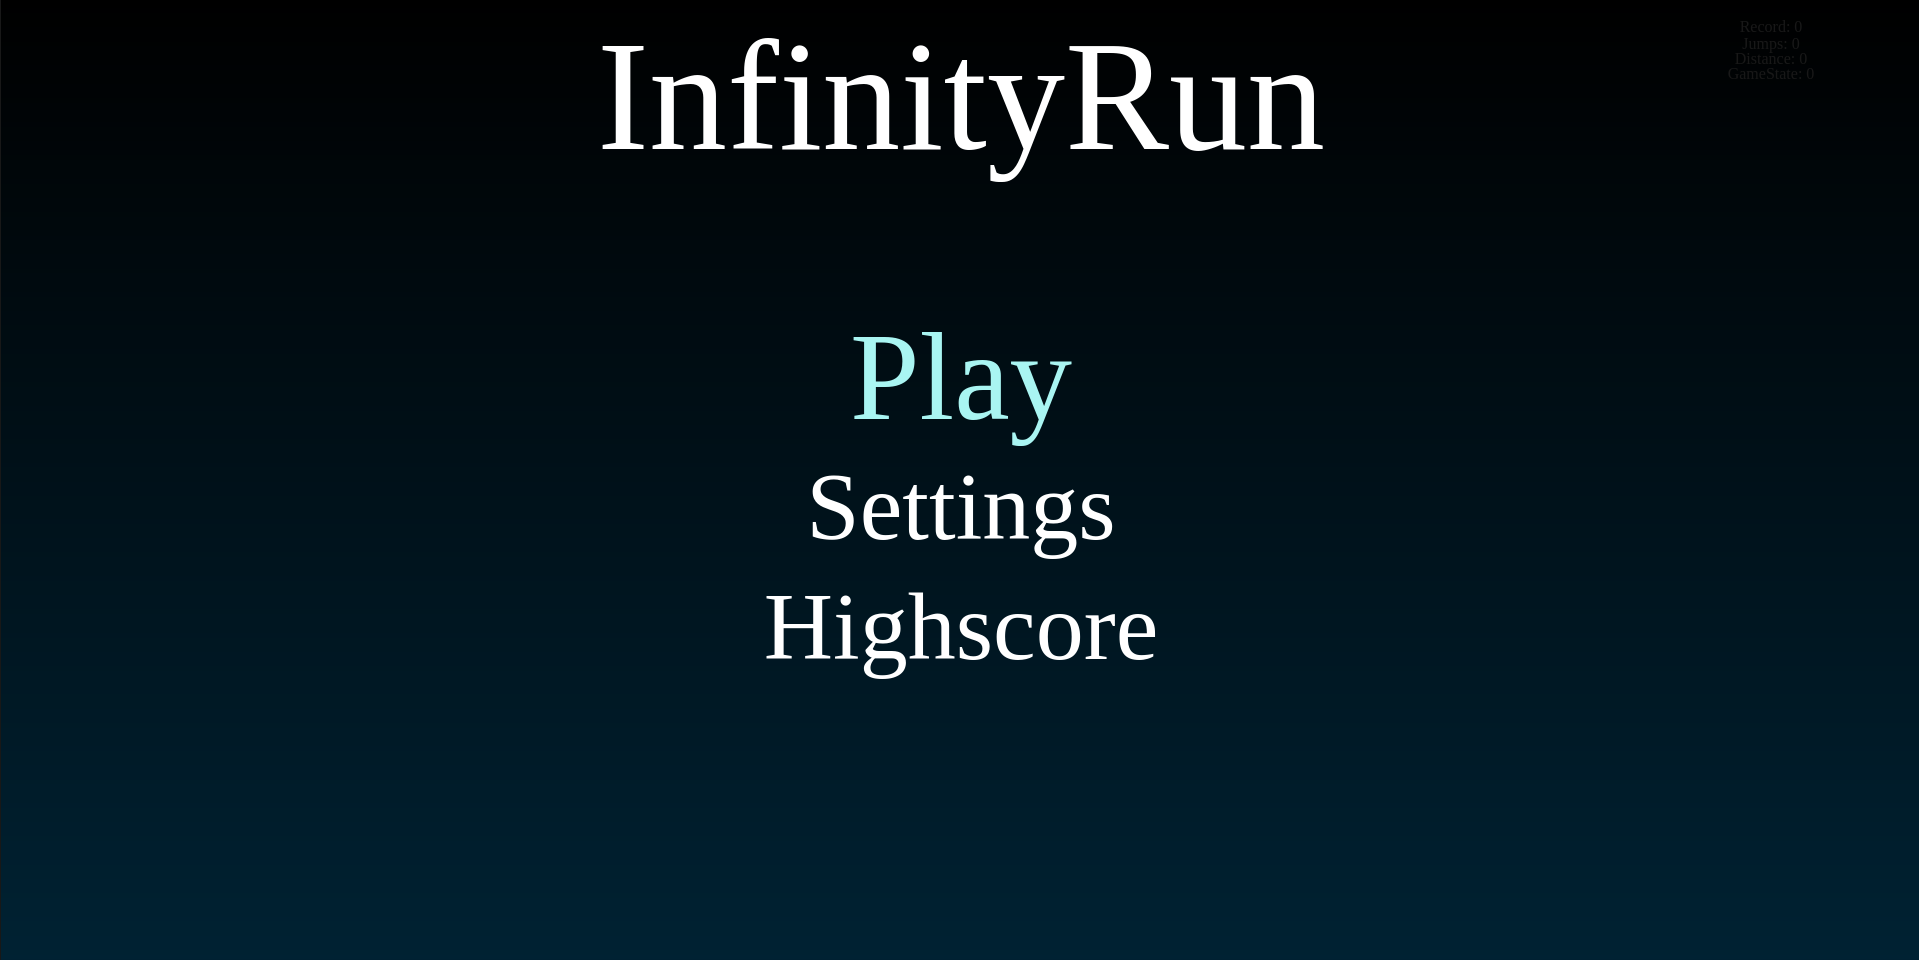
\includegraphics[scale=0.22]{content/pictures/start.png}
	\caption{Startbildschirm}
	\label{pic:start}
\end{figure}
\begin{figure}[htb]
	\centering
	
\includegraphics[scale=0.22]{content/pictures/spiel.png}
	\caption{Das Spiel}
	\label{pic:spiel}
\end{figure}
\newpage
\subsection{Bibliothek}
Bei der Erstellung des Spiels greifen wir auf eine JavaScript Bibliothek namens ``Sketch.js'' zurück.
Das Sketch.js Framework ermöglicht es uns, den Code vereinfacht und lesbarer zu schreiben. 
Beispiel wie Sketch.js funktioniert:

\lstset{language=java}
\begin{lstlisting}[frame=single]
function start() 
{
	context.now = +new Date();
    context.running = true;
}
        
function stop() 
{
	context.running = false;
}
        
function toggle() 
{       
	( context.running ? stop : start )();
}
        
function clear() 
{        
	if ( is2D )
        context.clearRect( 0, 0, context.width, context.height );
}
\end{lstlisting}
Quelle: \cite{sketch}
\subsection{Code}
\subsubsection{Framework initialisieren}
Hier in dieser Funktion wird ein Canvas-Element erstellt, dies geschieht mithilfe des Sketch-Frameworks. Dabei werden Eigenschaften wie die H\"ohe und Breite der Zeichenfl\"ache \"ubergeben.
\lstset{language=java}
\begin{lstlisting}[frame=single]
var InfinityRun = Sketch.create({
fullscreen: true,
width: 640,
height: 360,
container: document.getElementById('container')
});
\end{lstlisting}
\subsubsection{Spieler initialisieren}
In der Player-Update-Funktion wird der Player also unsere Spielfigur aktualisiert. Damit die Schwerkraft gegeben ist, wird zuerst die Y-Geschwindigkeit um eins erhöht. Hierbei ist zu beachten, dass die Y- Koordinatenachse nach unten zeigt.Danach wird die Position des Spielers neu festgesetzt. Für den Fall, dass der Spieler verliert, welches mittels if-Entscheidung überprüft wird, werden dann anschließend sämtliche Spielwerte auf ihren Ausgangswert zurückgesetzt. Als letztes wird überprüft ob der Spieler eine Taste gedrückt um zu Springen. Falls ja und er sich nicht schon in der Luft befindet wird die Y-Geschwindigkeit in die negative Richtung erhöht und die Spielfigur springt.
\lstset{language=java}
\begin{lstlisting}[frame=single]
Player.prototype.update = function() {
// Gravity 
this.velocityY += 1;
this.setPosition(this.x + this.velocityX, this.y + this.velocityY);

if (this.y > InfinityRun.height || this.x + this.width < 0) 
{
	this.x = 150;
	this.y = 50;
	this.velocityX = 0;
	this.velocityY = 0;
	InfinityRun.jumpCount = 0;
	InfinityRun.acceleration = 0;
	InfinityRun.accelerationTweening = 0;
	InfinityRun.scoreColor = '#181818';
	InfinityRun.platformManager.maxDistanceBetween = 350;
	InfinityRun.platformManager.updateWhenLose();
}

if ((InfinityRun.keys.UP || InfinityRun.keys.SPACE || InfinityRun.keys.W || InfinityRun.dragging) && this.velocityY < -8) 
{
	this.velocityY += -0.75;
}
};
\end{lstlisting}
\subsubsection{Erstellen der Spielebene}
In unserem Plattform-Manager werden die Plattformen initialisiert. Hierbei wird ein Wert ''maxDistanceBetween'' festgelegt. Ebenso werden mögliche Farben für die Plattformen gespeichert. Anschließend werden den ersten 3 Plattformen ihre Werte zugeordnet. Die erste Plattform hat hierbei feste Werte, damit der Spieler nicht sterben kann, am Anfang des Spiels. Die beiden nächsten Plattformen werden dann mit zufälligen Werten erstellt. Zum Schluss bekommt jede Plattform noch eine Höhe und Farbe zugeordnet.
\lstset{language=java}
\begin{lstlisting}[frame=single]
Player.prototype.update = function() {
function PlatformManager() 
{

	this.maxDistanceBetween = 300;

	this.colors = ['#2ca8c2', '#98cb4a', '#f76d3c', '#f15f74', '#5481e6'];

//first 3 Platforms execept the Starter Platform
	this.first = new Platform({
	x: 300,
	y: InfinityRun.width / 2,
	width: 400,
	height: 70
})

this.second = new Platform
({
	x: (this.first.x + this.first.width) + random(this.maxDistanceBetween - 150, this.maxDistanceBetween),
	y: random(this.first.y - 128, InfinityRun.height - 80),
	width: 400,
	height: 70
})

this.third = new Platform
({
	x: (this.second.x + this.second.width) + random(this.maxDistanceBetween - 150, this.maxDistanceBetween),
	y: random(this.second.y - 128, InfinityRun.height - 80),
	width: 400,
	height: 70
})
	this.first.height = this.first.y + InfinityRun.height;
	this.second.height = this.second.y + InfinityRun.height;
	this.third.height = this.third.y + InfinityRun.height;
	this.first.color = randomChoice(this.colors);
	this.second.color = randomChoice(this.colors);
	this.third.color = randomChoice(this.colors);
	this.colliding = false;
	this.platforms = [this.first, this.second, this.third];
}
\end{lstlisting}
\subsubsection{Update der Plattformen}
Die Plattform-Update-Funktion aktualisiert die 3 Plattformen. Sie hat zwei Aufgaben. Als erstes wird die Plattform immer, in Abhängigkeit zur Spielbeschleunigung, nach um drei nach links verschoben. Danach wird abgefragt, ob die Plattform schon ganz links aus dem Bild heraus gewandert ist und falls ja werden sämtliche Werte so zufällig neu gesetzt, dass sie wieder von rechts ins Bild laufen kann. Dies wird für alle 3 Plattformen gleich durchgeführt.
\lstset{language=java}
\begin{lstlisting}[frame=single]
PlatformManager.prototype.update = function() 
{
	this.first.x -= 3 + InfinityRun.acceleration;
	if (this.first.x + this.first.width < 0) 
	{
		this.first.width = random(450, InfinityRun.width + 200);
		this.first.x = (this.third.x + this.third.width) + random(this.maxDistanceBetween - 150, this.maxDistanceBetween);
		this.first.y = random(this.third.y - 32, InfinityRun.height - 80);
		this.first.height = this.first.y + InfinityRun.height + 10;
		this.first.color = randomChoice(this.colors);
	}

	this.second.x -= 3 + InfinityRun.acceleration;
	if (this.second.x + this.second.width < 0) 
	{
		this.second.width = random(450, InfinityRun.width + 200);
		this.second.x = (this.first.x + this.first.width) + random(this.maxDistanceBetween - 150, this.maxDistanceBetween);
		this.second.y = random(this.first.y - 32, InfinityRun.height - 80);
		this.second.height = this.second.y + InfinityRun.height + 10;
		this.second.color = randomChoice(this.colors);
	}

	this.third.x -= 3 + InfinityRun.acceleration;
	if (this.third.x + this.third.width < 0) 
	{
		this.third.width = random(450, InfinityRun.width + 200);
		this.third.x = (this.second.x + this.second.width) + random(this.maxDistanceBetween - 150, this.maxDistanceBetween);
		this.third.y = random(this.second.y - 32, InfinityRun.height - 80);
		this.third.height = this.third.y + InfinityRun.height + 10;
		this.third.color = randomChoice(this.colors);
	}
};
\end{lstlisting}
\subsubsection{Update der Plattformen}
In folgender Funktion werden mithilfe einer for-Schleife zuerst alle drei Plattformen abgefragt, ob diese, anhand von: "if(this.player.intersects..) " den Spieler ber\"uhren. Falls der Spieler eine Plattform ber\"uhrt, in diesem Fall " this.collidedPlatform.... " als Beispiel die zweite Plattform im Spiel ber\"uhrt, so wird der Variable "collidedPlatform" ein Objekt der zweiten Plattform zugewiesen. Außerdem wird zus\"atzlich noch die Y-Koordinate des Spielers auf die der Plattform gesetzt, was hier die Funktion " this.player.y < this.platformManager...." ist. Zus\"atzlich wird wenn die Y-Koordinate des Spielers und die Y-Koordinate der Plattform \"ubereinstimmen, die "velocityY" auf 0 gesetzt, was zur Folge hat, dass der Spieler nicht mehr f\"allt. Anschließend sollen die Partikel des Spielers die Farbe der Plattormen annehmen.
\lstset{language=java}
\begin{lstlisting}[frame=single]
    for (i = 0; i < this.platformManager.platforms.length; i++) 
    {
		if (this.player.intersects(this.platformManager.platforms[i])) 
		{
			this.collidedPlatform = this.platformManager.platforms[i];
			if (this.player.y < this.platformManager.platforms[i].y) 
			{
				this.player.y = this.platformManager.platforms[i].y;
				// Gravity after Collision with Platform
				this.player.velocityY = 0;
			}

			this.player.x = this.player.previousX;
			this.player.y = this.player.previousY;
			
			this.particles[(this.particlesIndex++) % this.particlesMax] = new Particle({
			x: this.player.x,
			y: this.player.y + this.player.height,
			color: this.collidedPlatform.color
});
\end{lstlisting}
\subsection{Nächste Ziele}
Da die Grundlegenden Spielfunktionen implementiert sind wollen wir uns in der zweiten Phase der Implementation nun auf das Design und die Effektsounds konzentrieren.
\section{Implementation - Endstand}
\subsection{Spielkonzept Änderungen}
Folgende Spielkonzept Äbnderungen haben wir im laufe der Implementation vorgenommen:
\begin{itemize}
	\item Die Spielebene hat anstatt Hindernisse Zufalls generierte variable Plattformen.
	\item Spiel-Menü eingefügt
	\item Spielhintergrund
\end{itemize}
\subsection{Funktionsdiagramm}
\begin{landscape}
	\begin{figure}%[hb]
		\centering
		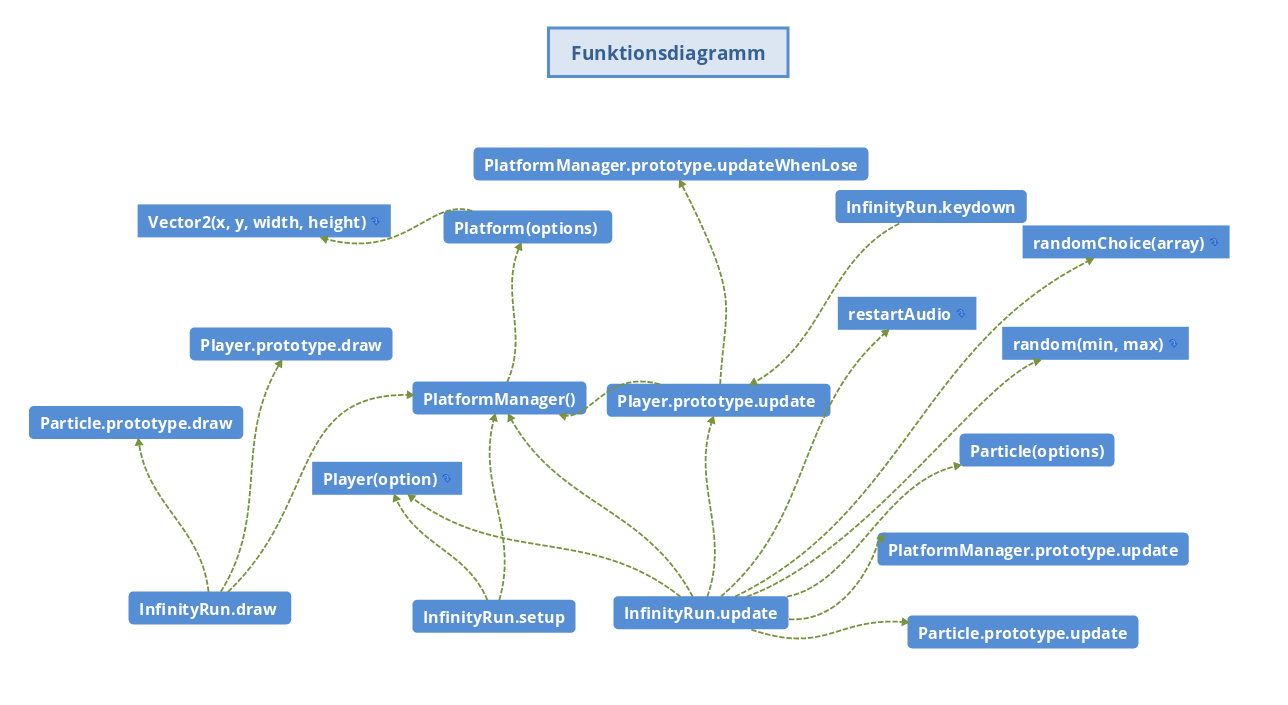
\includegraphics[scale=0.5]{content/pictures/funktionsdiagramm.png}
		\caption{Funktionsdiagramm}
		\label{pic:diagramm}
	\end{figure}
\end{landscape}
Beschreibung der Funktionen aus Abbildung \ref{pic:diagramm}
\begin{table}[h]
	\begin{tabular}{|l|l|}
		\toprule
		\textbf{Funktion}& \textbf{Erklärung}\\
		\midrule
		InfinityRun.draw & Spielfläche wird gezeichnet	\\ 
		InfinityRun.setup & Grundeinstellungen des Spiels	\\
		InfinityRun.update & Aktualisierung der Spielfläche	\\ 
		Particle.prototype.update & Aktualisierung der Partikel	\\ 
		PlatformManager.prototype.update & Neue Position der Plattformen	\\ 
		Particle(Option) & Einstellungen der Partikel	\\ 
		random(min, max) & Erstellen der Zufallszahl\\
		randomChoice(array) & Zufälliger Wert aus dem Array	\\
		restartAudio & Neustand der Audiosequenz	\\
		InfinityRun.keydown & Festlegung der Spieltasten	\\
		PlatformManager.prototype.updateWhenLose & Setzt die Plattformen zurück	\\
		Player.prototype.update & Aktualisierung der Spielfigur	\\
		PlatformManager() & Verwalten der Plattformen	\\
		Platform(options) & Erzeugt eine Plattform	\\
		Player(option) & Erstellt die Spielfigur	\\
		Vector2(x, y, width, height) & Verwaltungen der Koordinaten	\\
		Player.prototype.draw & Zeichnen der Spielfigur	\\
		Particle.prototype.draw & Zeichnen der Partikel	\\
		\bottomrule
	\end{tabular}
	\caption{Funktionsbeschreibung}
\end{table}
\subsection{Grafiken}
\subsubsection{Spiel}
Derzeit haben wir keine Grafiken implementiert, da unsere Objekte und Hintergründe mittels Canvas gezeichnet werden.
\subsubsection{Logo}
Wir haben für unser Spiel zusätzlich ein Logo erstellt dieses Logo wurde mit Gimp erstellt und wird in unserem Spiel, wie auch auf dem Deckblatt dieser Dokumentation angezeigt.
\begin{figure}[htb]
	\centering
	
\includegraphics[scale=1]{../../image/logo.png}
	\caption{Logo}
	\label{pic:logo}
\end{figure}
\newpage
\subsection{Code Änderungen}
\subsubsection{Musik}
Die ausgewählte Musik wurde per Audio-Element in JavaScript implementiert. Es gibt zwei Audio-Elemente, einen für den Hintergrund und einen für die Effekte. Folgende Code Beispiele zeigen diese Elemente.\\
Erstellen der Audio-Elemente:
\lstset{language=java}
\begin{lstlisting}[frame=single]
var bgaudio = document.getElementById('backgroundmusic');
var fxaudio = document.getElementById('fxaudio');
\end{lstlisting}
Zugriff auf Element per Funktion zum Neustarten der Musik:
\lstset{language=java}
\begin{lstlisting}[frame=single]
function restartAudio() 
{
	// Check for audio element support.
	if (window.HTMLAudioElement) 
	{
		try 
		{                     
			// Tests the paused attribute and set state. 
			if (bgaudio.ended) 
			{
				bgaudio.currentTime = 0;
				bgaudio.play();
			}                    
		}
		catch (e) 
		{
			// Fail silently but show in F12 developer tools console
			if(window.console && console.error("Error:" + e));
		}
	}
}
\end{lstlisting}
Beispiel für die Audio Wiedergabe:
\lstset{language=java}
\begin{lstlisting}[frame=single]
if (this.dragging || this.keys.SPACE || this.keys.UP || this.keys.W) 
{
	this.player.velocityY = this.player.jumpSize;
	this.jumpCount++;
	fxaudio.pause();
	fxaudio.src = 'sounds/jump.wav';
	fxaudio.load();
	fxaudio.play();	
}
\end{lstlisting}
\newpage
\subsubsection{Hintergrund}
Unser Hintergrund stellt in drei verschiedenen Layern Hochhäuser dar. Diese Hochhäuser werden ähnlich wie unsere Plattformen generiert und von links nach rechts auf dem Bildschirm dargestellt. Der Hintergrund reagiert zusätzlich auf Sprünge der Spielfigur.
Erstellt die Hochhäuser mit ihren Eigenschaften:
\begin{lstlisting}[frame=single]
Street.prototype.populate = function() 
{
	var newHeight, newWidth, results, totalWidth;
	totalWidth = 0;
	results = [];
	while (totalWidth <= InfinityRun.width + (this.width.max * 2)) 
	{
		newWidth = round(random(this.width.min, this.width.max));
		newHeight = round(random(this.height.min, this.height.max));
		this.alltowers.push(new Tower({
			layer: this.layer,
			x: this.alltowers.length === 0 ? 0 : this.alltowers[this.alltowers.length - 1].x + this.alltowers[this.alltowers.length - 1].width,
			y: InfinityRun.height - newHeight,
			width: newWidth,
			height: newHeight,
			color: this.color
		}));
		results.push(totalWidth += newWidth);
	}
	return results;
};
\end{lstlisting}
Aktualisieren der Hochhäuser, für neues erscheinen am rechten Spielrand:
\begin{lstlisting}[frame=single]
Street.prototype.update = function() 
{
	var firstTower, lastTower, newHeight, newWidth;
	if (InfinityRun.accelerationTweening==0)
	{
		this.x-=((150) * this.speed) * dt;
	}
	else
	{
		this.x -= ((InfinityRun.accelerationTweening*330) * this.speed) * dt;
	}

	firstTower = this.alltowers[0];
	if (firstTower.width + firstTower.x + this.x < 0) 
	{
		newWidth = round(random(this.width.min, this.width.max));
		newHeight = round(random(this.height.min, this.height.max));
		lastTower = this.alltowers[this.alltowers.length - 1];
		firstTower.reset({
			layer: this.layer,
			x: lastTower.x + lastTower.width,
			y: InfinityRun.height - newHeight,
			width: newWidth,
			height: newHeight,
			color: this.color
		});
	return this.alltowers.push(this.alltowers.shift());
	}
};
\end{lstlisting}
\newpage
\subsection{Das Spiel - Endstand}
Hier werden zwei Screenshots des derzeitigen Spiels dargestellt. In der Abbildung \ref{pic:startende} zu sehen, ist der endgültige Startbildschirm des Spiels. Hier gibt es verschiedene Auswahlmöglichkeiten, die das Spielerlebnis ergänzen. In der Abbildung \ref{pic:spielende} zu sehen ist der endgültige Stand des Spiels. Der Hintergrund reagiert hierbei auf den Sprung des Spielers und ein Partikeleffekt hinter dem Spieler ist ebenfalls implementiert.
\begin{figure}[htb]
	\centering
	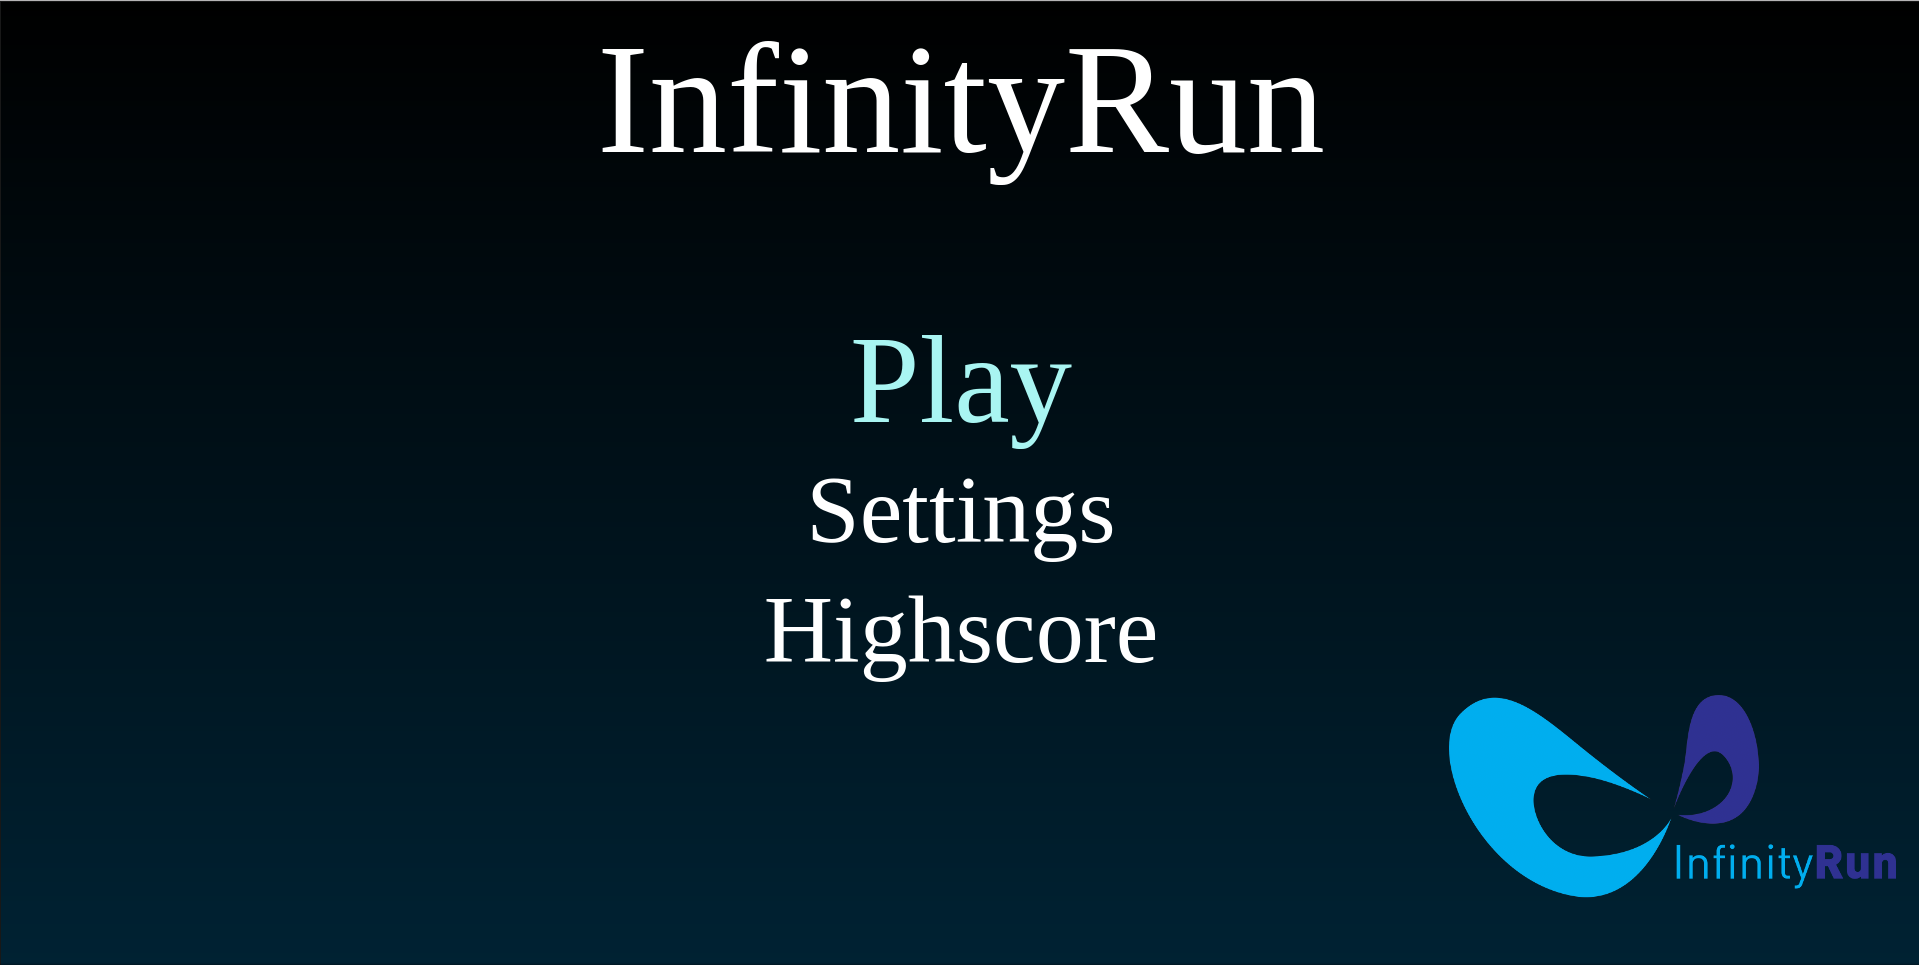
\includegraphics[scale=0.22]{content/pictures/startende.png}
	\caption{Startbildschirm - Endstand}
	\label{pic:startende}
\end{figure}
\begin{figure}[htb]
	\centering
	
\includegraphics[scale=0.22]{content/pictures/spielende.png}
	\caption{Das Spiel - Endstand}
	\label{pic:spielende}
\end{figure}
\newpage
\subsection{Sounds}
Bei den implementierten Spielsounds greifen wir auf eine freie Sounddatenbank zurück. Quelle: \cite{sounds}\\
Folgende Sounds werden wir verwenden:
\begin{table}[h]
	\centering
	\begin{tabular}{|l|l|}
		\toprule
		\textbf{Sounds}& \textbf{Links}\\
		\midrule
		Menu & \url{https://www.freesound.org/people/lharman94/sounds/329597/}\\ 
		Main1 & \url{https://www.freesound.org/people/nicolasdrweski/sounds/179684/}\\
		Main2  & \url{https://www.freesound.org/people/joshuaempyre/sounds/251461/}\\ 
		Main3  & \url{https://www.freesound.org/people/Flick3r/sounds/48544/}\\
		Main4 & \url{https://www.freesound.org/people/Flick3r/sounds/45623/}\\
		Jump & \url{https://www.freesound.org/people/Lefty_Studios/sounds/369515/}\\
		Level-Up & \url{https://www.freesound.org/people/n_audioman/sounds/275895/}\\
		Error & \url{https://www.freesound.org/people/SamsterBirdies/sounds/363920/}\\
		Crash & \url{https://www.freesound.org/people/n_audioman/sounds/276341/}\\
		\bottomrule
	\end{tabular}
	\caption{Sound Links}
\end{table}
%\section{Test}
%\subsection{Testplan}
%\begin{table}[h]
%	\centering
%	\begin{tabular}{|c|l|l|}
%		\toprule
%		\textbf{Test-Nr.}& \textbf{Beschreibung}& Fehler \\
%		\midrule
%		1 & Test &\\ 
%		2 & Test &\\
%		3 & Test &\\ 
%		4 & Test &\\
%		5 & Test &\\
%		\bottomrule
%		\end{tabular}
%		\caption{Testplan}
%\end{table}
%\section{Dokumentation \& Pr\"asentation}


%\chapter{[Eigene Kapitel]}
%\chapter{Ausblick}
In der Zukunft könnte das Spiel zusätzliche Schwierigkeitsgrade, eine Auswahl von Spielfiguren, ein Umgekehrter Spielverlauf und einen Globalen Score der bei Neustart verfügbar ist könnte implementiert werden. Wir haben uns bis zum derzeitigen Stand des Spiels rein um das Grundspiel und die Stabilität gekümmert, somit blieben solche ``Nice to have'' Features aus. Zusätzlich könnte dieses Spiel vor allem auf mobilen Plattformen als App Angeboten werden können.
%\chapter{Fazit}
Der Informatik Workshop hat uns gezeigt, dass Teamwork eine der wichtigsten Eigenschaften einer solchen Projektarbeit ist. Wir haben gelernt gemeinsam an einem Strang zu ziehen und hatten keinerlei Probleme unseren Projektplan einzuhalten. Trotz Problemen bei der Umsetzung des Spiel konnten wir wie geplant alle Features implementieren. Das Verwenden von Github erleichterte das Arbeiten im Team ungemein, so konnten wir parallel an Doku und Spiel arbeiten. Abschließend können wir sagen, dass wir ein nettes kleines Spiel auf die Beine gestellt haben.

% Schalgwortverzeichnis (Index)
%\printindex

% Literaturverzeichnis
\singlespacing
\bibliographystyle{alphadin}
\bibliography{bibtex}

% Eidesstattliche Erklärung
\chapter*{Eidesstattliche Erklärung\markboth{Eidesstattliche Erklärung}{}}
% Eintrag in das Inhaltsverzeichnis 
\addcontentsline{toc}{chapter}{Eidesstattliche Erklärung}

Wir versichern, dass wir die vorstehende Arbeit selbständig verfasst und hierzu
keine anderen als die angegebenen Hilfsmittel verwendet haben. Alle Stellen der Arbeit die 
wörtlich oder sinngemäß aus fremden Quellen entnommen wurden, sind als solche kenntlich gemacht.
\\
\\
Die Arbeit wurde bisher in gleicher oder ähnlicher Form in keinem anderen
Studiengang als Prüfungsleistung vorgelegt oder an anderer Stelle
veröffentlicht.
\\
\\
Uns ist bewusst, dass eine falsche Erklärung rechtliche Folgen haben kann.

\vspace*{1.5cm} \par
\line(1,0){350} \par
\docOrt, den  \docAbgabedatum ~~\docErsterReferent\\\\
\vspace*{1.5cm} \par
\line(1,0){350} \par
\docOrt, den  \docAbgabedatum ~~\docZweiterReferent\\\\
\vspace*{1.5cm} \par
\line(1,0){350} \par
\docOrt, den  \docAbgabedatum ~~\docDritterReferent\\\\
\vspace*{1.5cm} \par
\line(1,0){350} \par
\docOrt, den  \docAbgabedatum ~~\docVierterReferent\\\\
\vspace*{1.5cm} \par
\line(1,0){350} \par
\docOrt, den  \docAbgabedatum ~~\docFuenfterReferent


\appendix
% Hier können Anhaenge angefuegt werden
\chapter{Anhang}
\section{Github Changelog}
Der Changelog wird aus unseren Github Commits per Befehl exportiert. Derzeit ist die Quelle nicht einsehbar, da das Repository auf dem wir arbeiten auf ``Private'' gesetzt ist. Zur endgültigen Abgabe wird dieses natürlich Veröffentlicht.
\lstset{language=bash}
\begin{lstlisting}[frame=single]
$ git log --pretty=tformat:'%h %<(13)%an %cd %s%n' --date=short > CHANGELOG.md
\end{lstlisting}
Quelle: \cite{changelog}
\begin{table}[h]
	\centering
	\begin{tabular}{|l|l|}
		\toprule
		\textbf{Github}& \textbf{Name}\\
		\midrule
		Slay3r & Florian Durli 	\\ 
		r4qtor & Marco Maier	\\
		butjo  & Johannes But	\\ 
		ans77  & Jannik Ivosevic\\
		Krusher999 & Koray Emtekin\\
		\bottomrule
	\end{tabular}
	\caption{Github Namen}
\end{table}
\\\\
\textbf{Changelog: }
\lstset{
	literate={ö}{{\"o}}1
	{ä}{{\"a}}1
	{ü}{{\"u}}1
}
\lstinputlisting{../../CHANGELOG.md}
\section{game.js}
\lstinputlisting{../../js/game.js}
\section{game.css}
\lstinputlisting{../../css/game.css}
\section{index.html}
\lstinputlisting{../../index.html}
\end{document}